The last prototype developed for TRITIUM was TRITIUM-IFIC 2, marked as A in Figure \ref{fig:TritiumIFIC2}. This prototype, built in the IFIC workshop, consists of a cylindrical Teflon vessel, shown in Figure \ref{fig:Tritium-IFIC2_vessels}, with a similar shape to that of the TRITIUM-Aveiro prototype. The internal length and diameter of the Teflon vessel were $210~\mm$ and $36~\mm$ respectively. This prototype contains $800$ uncladded BCF-12 scintillating fiber of $200~\mm$ length. This number is larger than that of the TRITIUM-Aveiro prototype and is contained in a smaller volume. The fibers used were cleaved, polished and cleaned with the conditioning process described in section \ref{sec:CharacterizationScintillatingFibers}. This number of fibers, which were freely arranged, just allowed water to flow through them. Two PMMA windows, located at the ends of the fiber bundle, allowed to read the scintillation light as in the TRITIUM-Aveiro prototype. 

\begin{figure}[h]
\centering
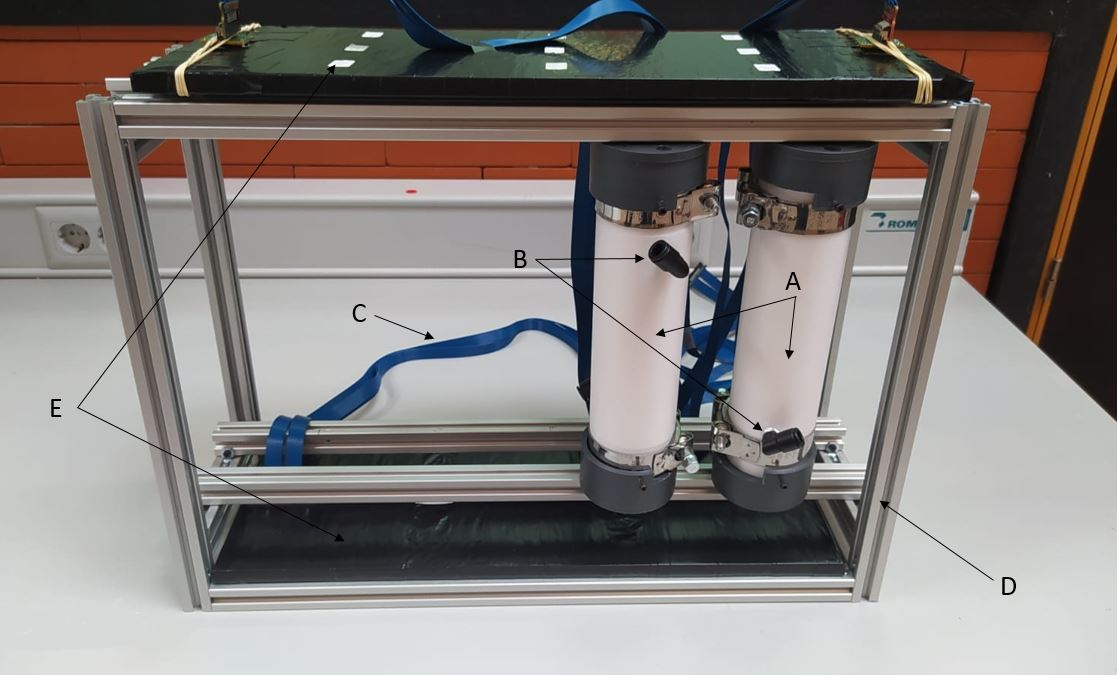
\includegraphics[scale=0.4]{5Prototypes/53FinalPrototypes/532TritiumIFIC2/Tritium_IFIC_2_full_module.jpg}
\caption{TRITIUM-IFIC 2 prototype and active veto within the metalic structure.\label{fig:TritiumIFIC2}}
\end{figure}

\begin{figure}
\centering
    \begin{subfigure}[b]{0.35\textwidth}
    \centering
    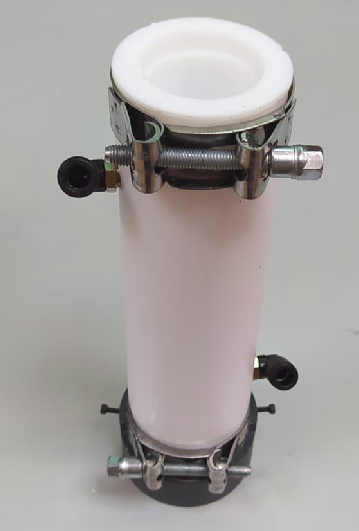
\includegraphics[width=\textwidth]{5Prototypes/53FinalPrototypes/532TritiumIFIC2/Tritium_IFIC_2_vessel1.png}  
    \caption{\label{subfig:Tritium_IFIC_2_vessel}}
    \end{subfigure}
    \hfill
    \begin{subfigure}[b]{0.3\textwidth}
    \centering
    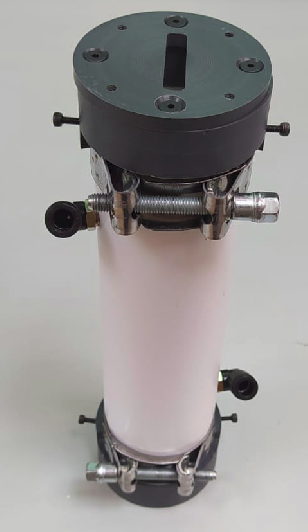
\includegraphics[width=\textwidth]{5Prototypes/53FinalPrototypes/532TritiumIFIC2/Tritium_IFIC_2_vessel2.png}  
    \caption{\label{subfig:TritiumIFIC2_vessel_with_PVC_caps}}
    \end{subfigure}
 \caption{a) TRITIUM-IFIC 2 Teflon vessel. b) TRITIUM-IFIC 2 Teflon vessel with PVC caps}
 \label{fig:Tritium-IFIC2_vessels}
\end{figure}

A $5~\mm$ width PMMA optical windows is sufficient to guarantee tightness, since the detector works at very low water pressure. Two clamps keep the tightness of the prototype, similar to the TRITIUM-Aveiro prototype. PMMA was chosen for its optical properties, especially its transmission coefficient, shown in Figure \ref{fig:PMMATransmissionSpectrum}, which was measured for visible spectrum in the ICMOL laboratories. This transmission coefficient is approximately $95\%$ for the working wavelength ($435~\nm$). Slightly better transmission coefficients can be achieved with other materials such as quartz or sapphire but they are much more expensive.

\begin{figure}[h]
\centering
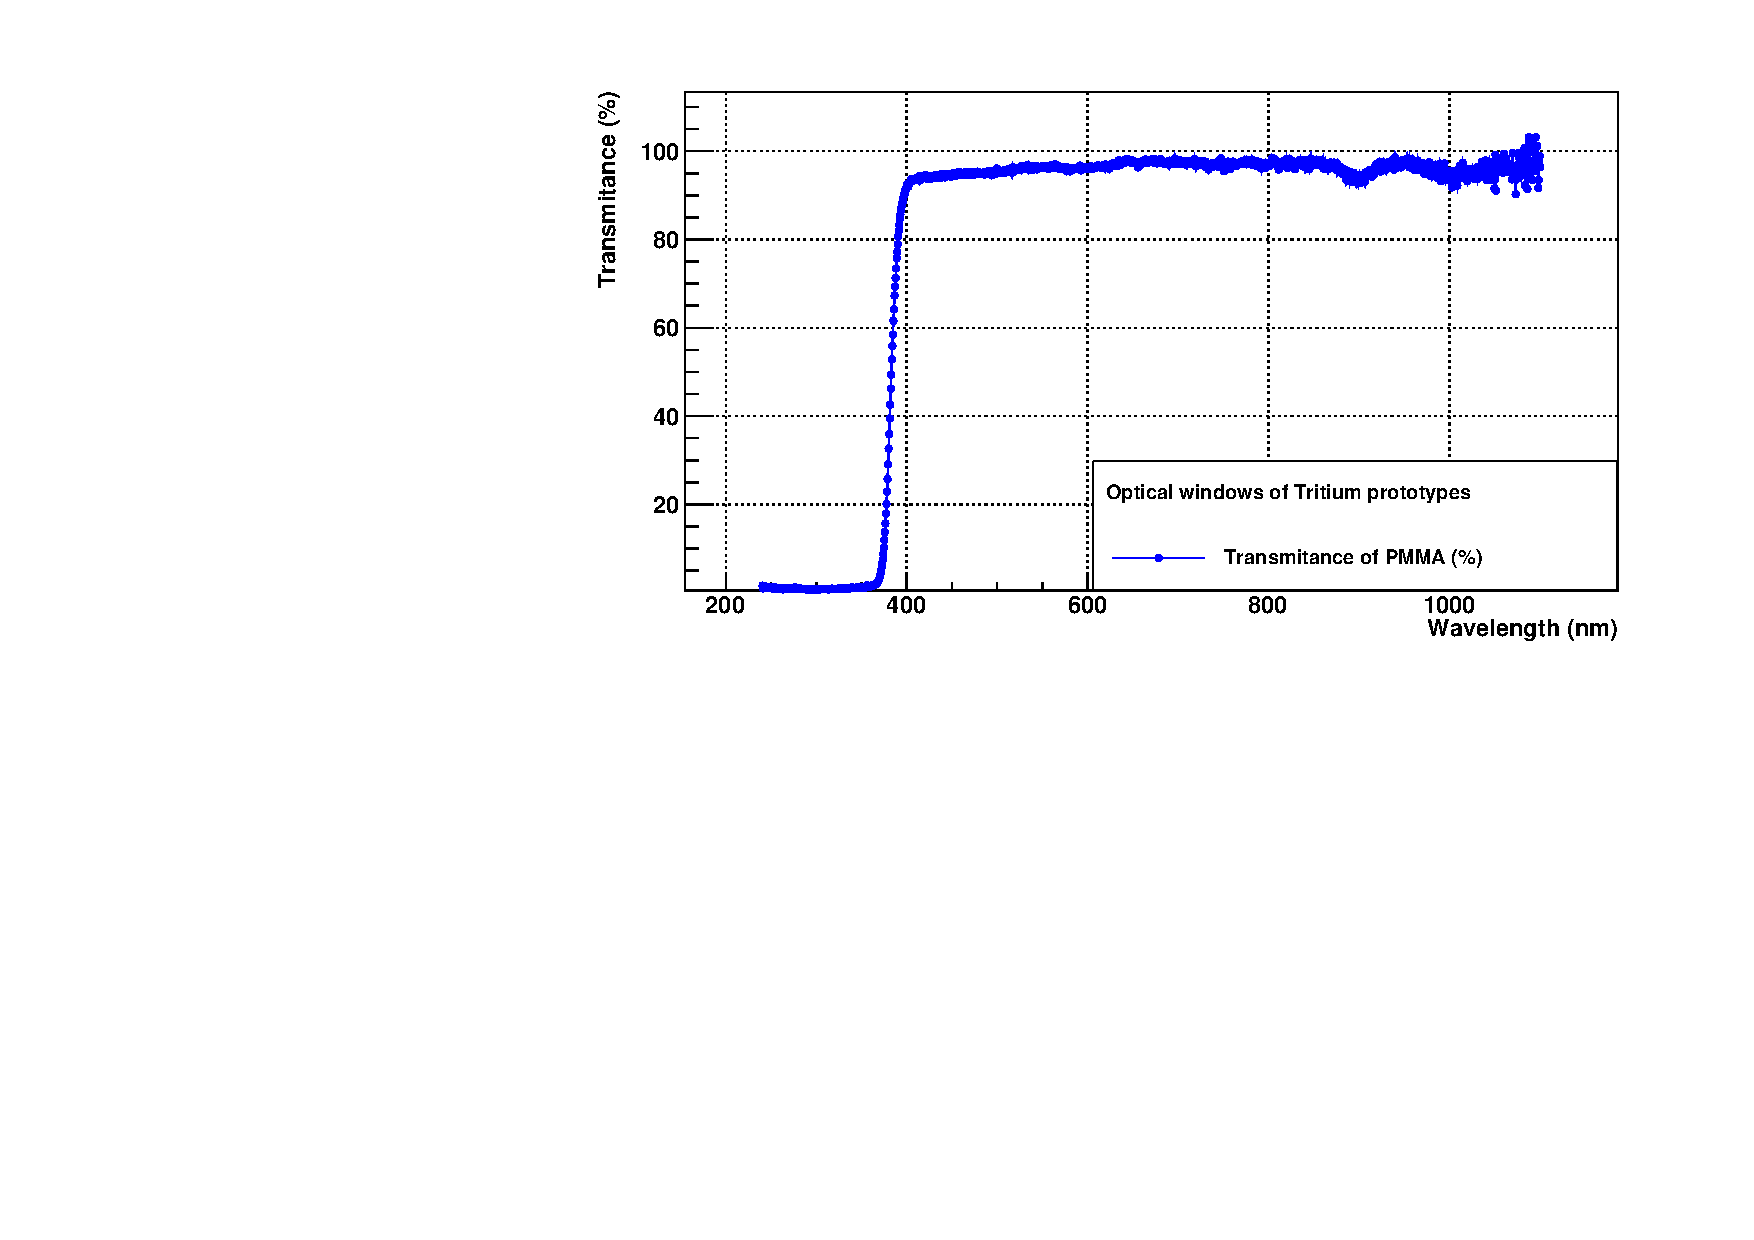
\includegraphics[scale=0.6]{5Prototypes/53FinalPrototypes/532TritiumIFIC2/TransmissionSpectrumPMMA_cut_at_low_energy.pdf}
\caption{Transmission spectrum of light by a $5~\mm$ thick of PMMA plate. (measured in the ICMOL laboratory). \label{fig:PMMATransmissionSpectrum}}
\end{figure}	

A water inlet/outlet was implemented in the Teflon vessel, shown in Figure \ref{fig:Tritium-IFIC2_vessels}, to allow a constant water flux, as in the TRITIUM-Aveiro prototype.

In the first laboratory measurements, two R8520-460 PMTs from the Hamamatsu Photonics \cite{DataSheetPMTs} were used to compare the results to those of the previous prototypes. However, measurements of the TRITIUM-IFIC 2 prototype with SiPM arrays controlled by PETSYS have already started, as the final version will use them. PETSYS has a graphical user interface, shown in Figure \ref{fig:GUI_PETSYS}. It allows remote controll of all the different options such as supply voltage for the SiPM arrays, thresholds, etc., via computer terminal. 

\begin{figure}[h]
\centering
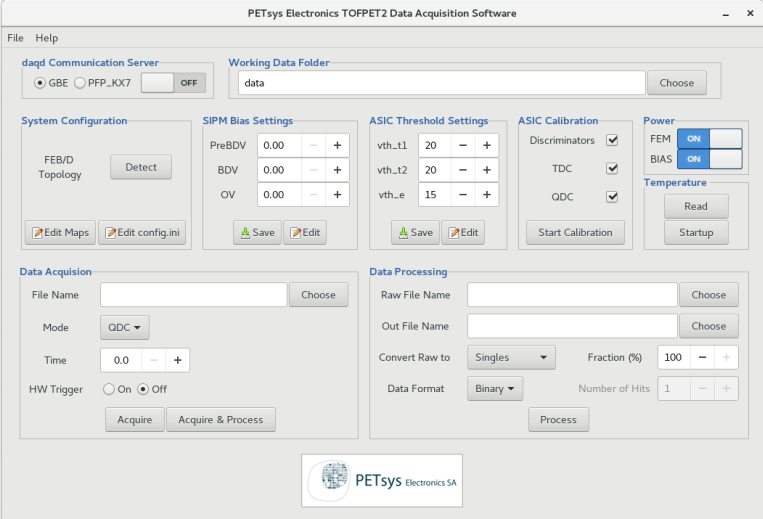
\includegraphics[scale=0.38]{5Prototypes/53FinalPrototypes/532TritiumIFIC2/GUI_PETSYS.png}
\caption{Graphical User Interface (GUI) of PETSYS.\label{fig:GUI_PETSYS}}
\end{figure}

Two PVC cañ.-s, located at both ends of the prototype were used to provide to the SiPMs a light-tight environment. An aluminum structure was designed and built to house up to 10 TRITIUM-IFIC 2 modules and two cosmic vetos, marked as D in Figure \ref{fig:TritiumIFIC2}.

The available space within the lead shield in Arrocampo site can accommodate up to 5 structures, which means that the final TRITIUM moitor may accommodate up to 50 TRITIUM-IFIC 2 modules and 5 different cosmic vetos. As the sensitivity of the TRITIUM monitor scales with the number of TRITIUM modules used, the results obtained with the TRITIUM monitor should improve those results by a factor of $\sqrt{N}$, where N is the number of modules used.

Two identical TRITIUM-IFIC 2 prototypes were built, as for the TRITIUM-IFIC 0 prototype. One of them was filled with pure water and used to measure the background and the other was filled with a radioactive liquid source of tritium and employed to measure the signal. The water volume in both cases was $82~\milli\liter$ (uncertainty of $0.05\%$).The activity of the tritium source used for this prototype was $10~\kilo\becquerel/\liter$ (uncertainty of $2.24\%$), which was prepared by diluting a sample of tritiated water in pure water. The signal and background energy spectra are shown in Figure \ref{subfig:SignalBackgroundEnergySpectraTritiumIFIC2}. The energy spectrum of tritium, Figure \ref{subfig:TritiumEnergySpectraTritiumIFIC2}, was obtained by substracting the background to the signal. The rates obtained from these three spectra are given in Table \ref{tab:CountsPerSecondTRITIUMIFIC2}. 

\begin{figure}
\centering
    \begin{subfigure}[b]{0.73\textwidth}
    \centering
    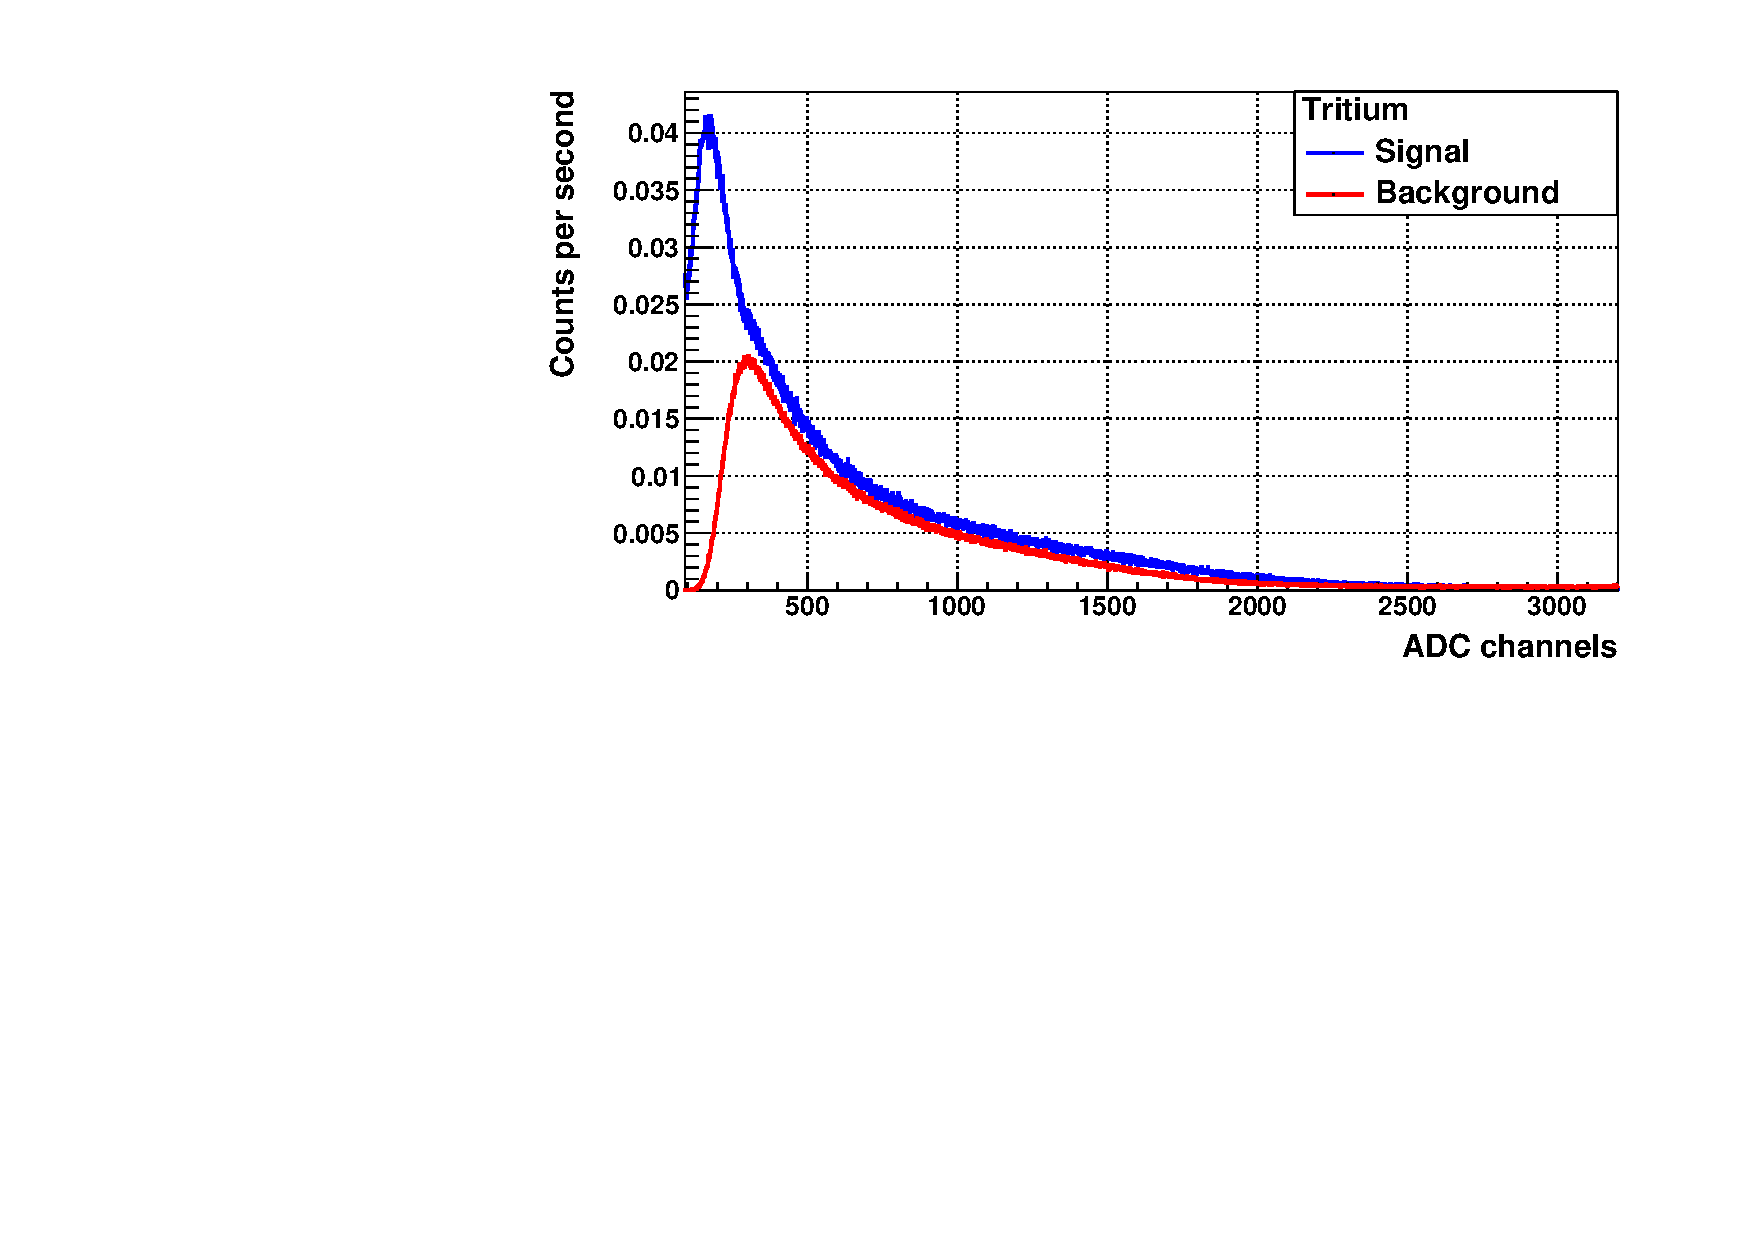
\includegraphics[width=\textwidth]{7ExperimentalResultsDetectors/71ExperimentalResultsLaboratory/714TRITIUMIFIC2/TritiumIFIC2SignalsHigherZOOM_NP.pdf}  
    \caption{\label{subfig:SignalBackgroundEnergySpectraTritiumIFIC2}}
    \end{subfigure}
    \hfill
    \begin{subfigure}[b]{0.73\textwidth}
    \centering
    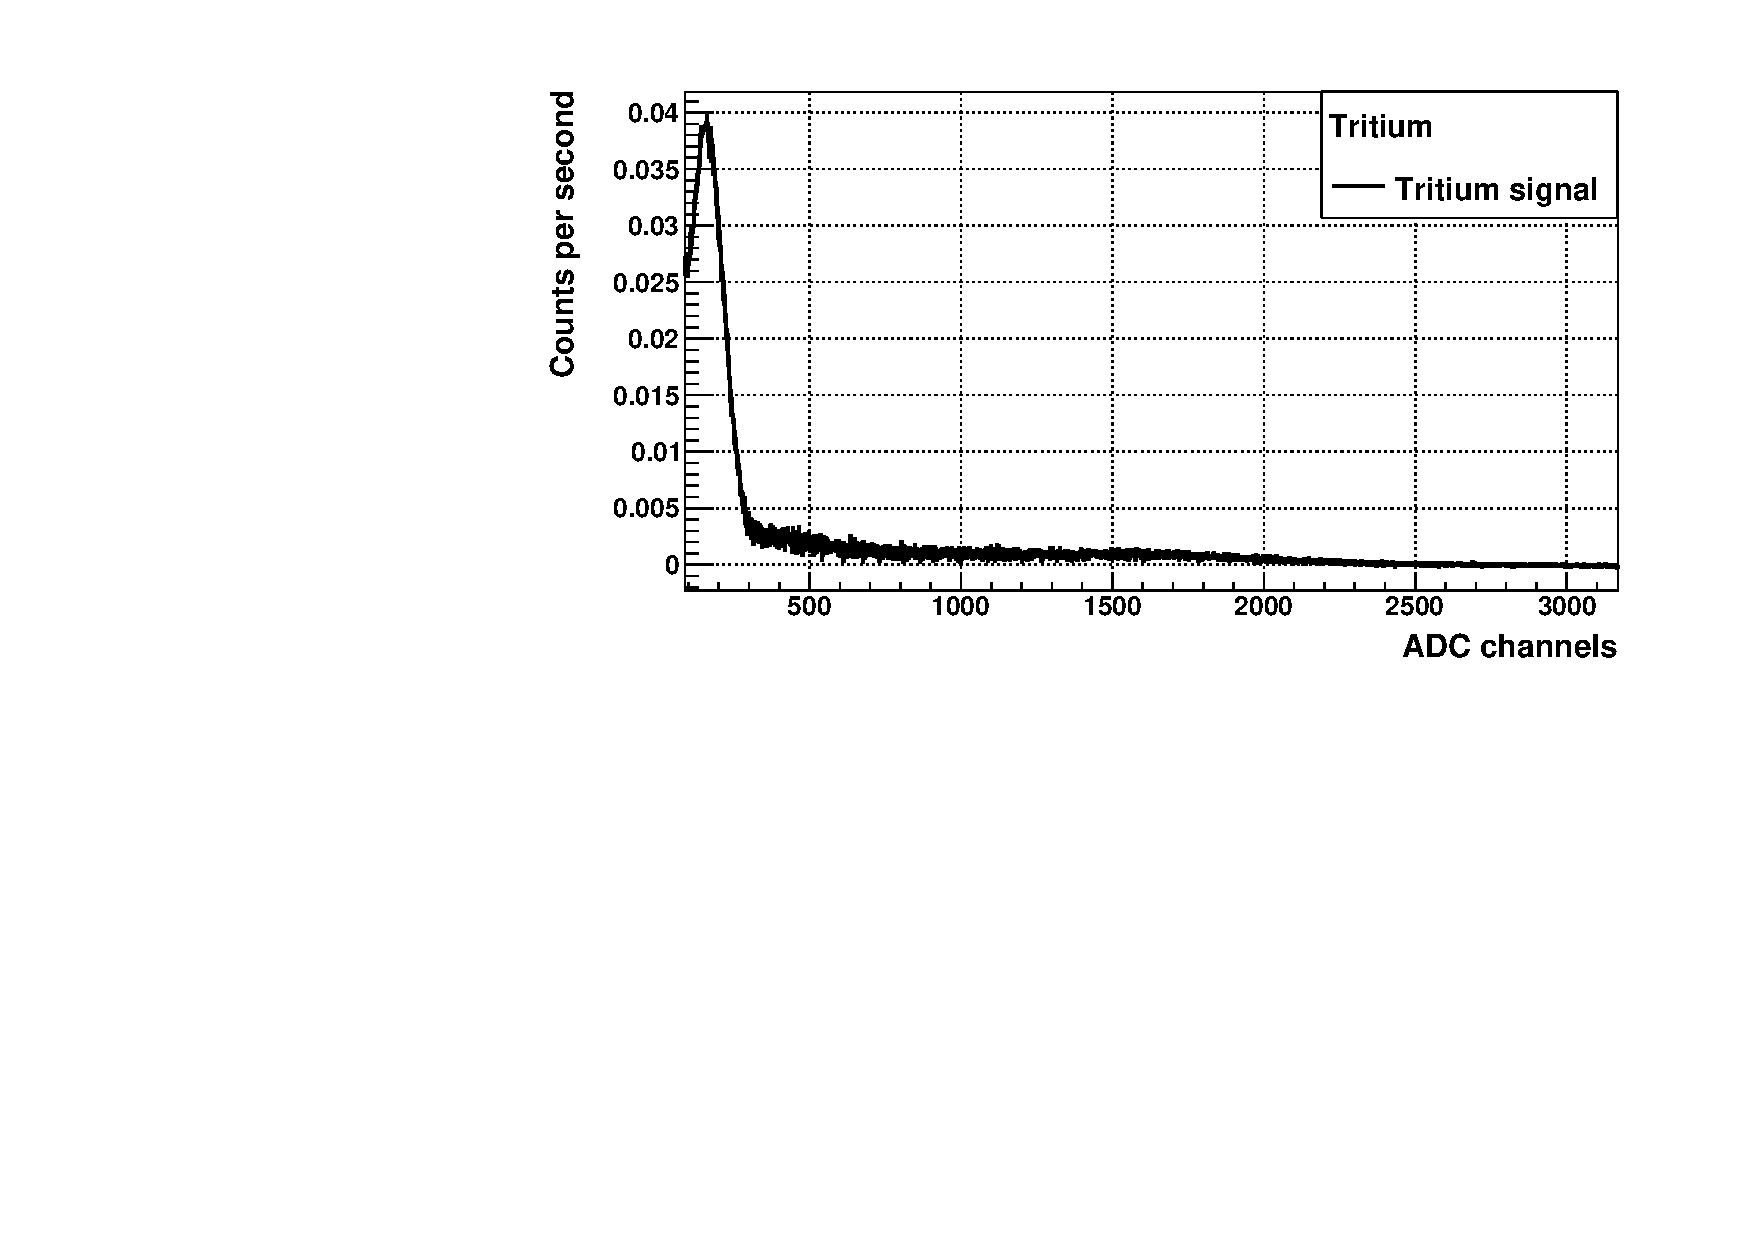
\includegraphics[width=\textwidth]{7ExperimentalResultsDetectors/71ExperimentalResultsLaboratory/714TRITIUMIFIC2/TritiumIFIC2ClearHigherZOOM_NP.pdf}  
    \caption{\label{subfig:TritiumEnergySpectraTritiumIFIC2}}
    \end{subfigure}
 \caption{Energy spectra measured with TRITIUM-IFIC 2 prototype. a) Signal and background energy spectra. b) Tritium energy spectrum.}
 \label{fig:EnergySpectraTRITIUMIFIC2}
\end{figure}

\begin{table}[htbp]
\centering{}%
\begin{tabular}{cc}
\toprule 
Spectrum & Counts/second \tabularnewline
\midrule
\midrule 
Signal prototype & $19.05 \pm 0.18$ \tabularnewline
Background prototype & $11.54 \pm 0.14$ \tabularnewline  
Tritium counts & $7.11 \pm 0.23$ \tabularnewline
\bottomrule
\end{tabular}
\caption{Counting rates measured by TRITIUM-IFIC 2 prototype.}
\label{tab:CountsPerSecondTRITIUMIFIC2}
\end{table}
The tritium detection efficiency obtained for this prototype is $(7.11 \pm 0.28)\cdot{} 10^{-1}~\liter\second^{-1}\kilo\becquerel^{-1}$. This efficiency is larger than those reported in the literature, Table \ref{tab:PlasticScinTritium}. This is an expected result since the active area of this prototype is the largest. To remove the active area effect, the specific efficiency was measured, obtaining a value of 
$$S=(1.59 \pm 0.48)\cdot{} 10^{-5}~\liter\second^{-1}\kilo\becquerel^{-1}\cm^{-2}$$
Again, it can be observed that this prototype has the largert specific efficiency reported for tritium detection.

The energy spectrum is given in ADC channels, since an energy calibration for a plastic scintillator is not accurate due to the large uncertainty in the number of photons produced per energy event. Nevertheless, a detector calibration in units of photons detected per event can be obtained from the single-photon distribution of the PMTs. The PMTs used to read this prototype was decoupled to the prototype and covered with a special black blanket to screen the PMT from external photons. The distribution measured fitted to a Gaussian function is shown in Figure \ref{subfig:SinglePhotonDistributionIFIC2}. As can be seen, the mean and uncertainty of the single photon signal are around $172$ and $66$ ADC channels, respectively, for one of the PMT and $173$ and $57$ ADC channels, respectively, for the other. The tritium signal given in number of photons detected per event, shown in Figure \ref{subfig:TritiumSignalTRITIUMIFIC2}, obtained as the ratio of the energy spectrum to the single-photon distribution mean. A maximum of $15$ photons are measured per tritium event.%, which is in agreement with the expected result taking in to account the efficiencies involved. 

\begin{figure}
\centering
    \begin{subfigure}[b]{0.73\textwidth}
    \centering
    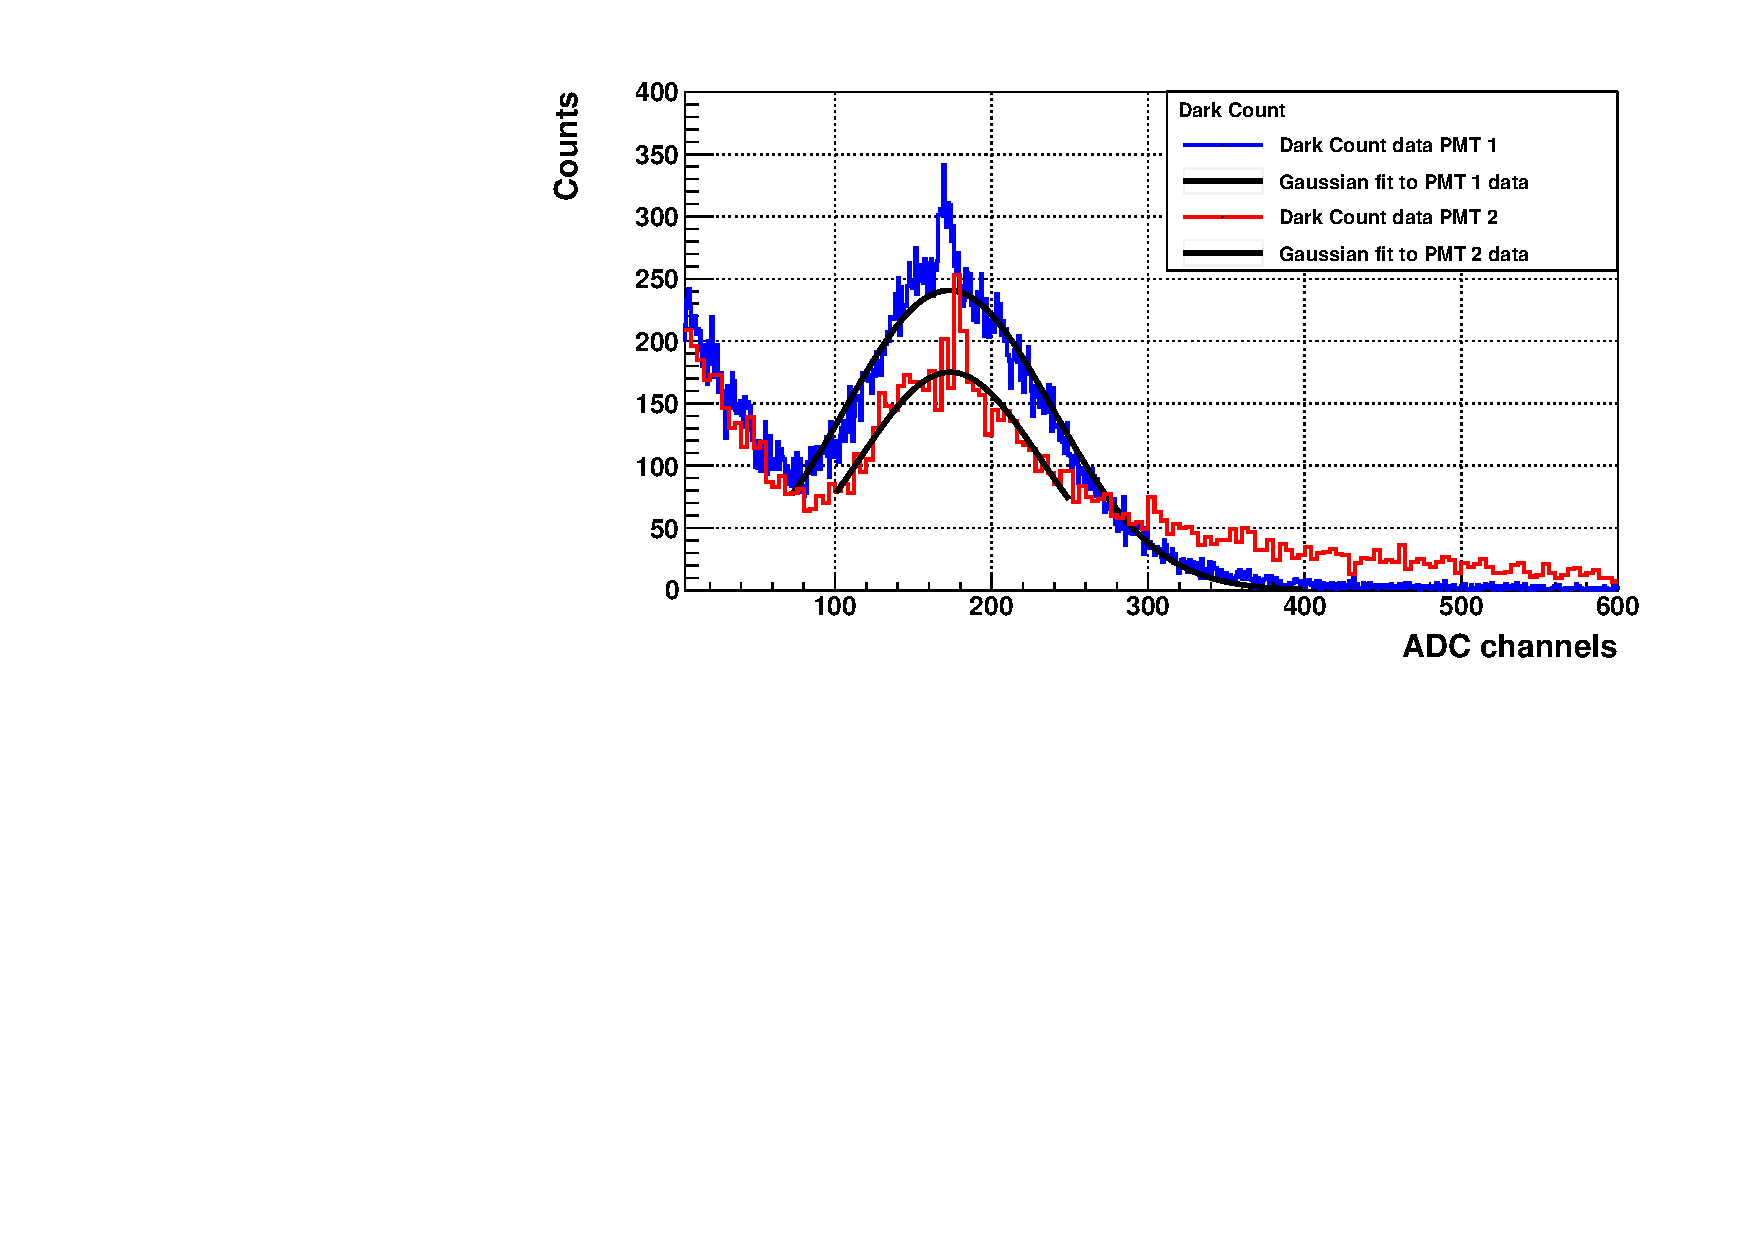
\includegraphics[width=\textwidth]{7ExperimentalResultsDetectors/71ExperimentalResultsLaboratory/714TRITIUMIFIC2/SinglePhotonDistribution2.pdf}  
    \caption{\label{subfig:SinglePhotonDistributionIFIC2}}
    \end{subfigure}
    \hfill
    \begin{subfigure}[b]{0.73\textwidth}
    \centering
    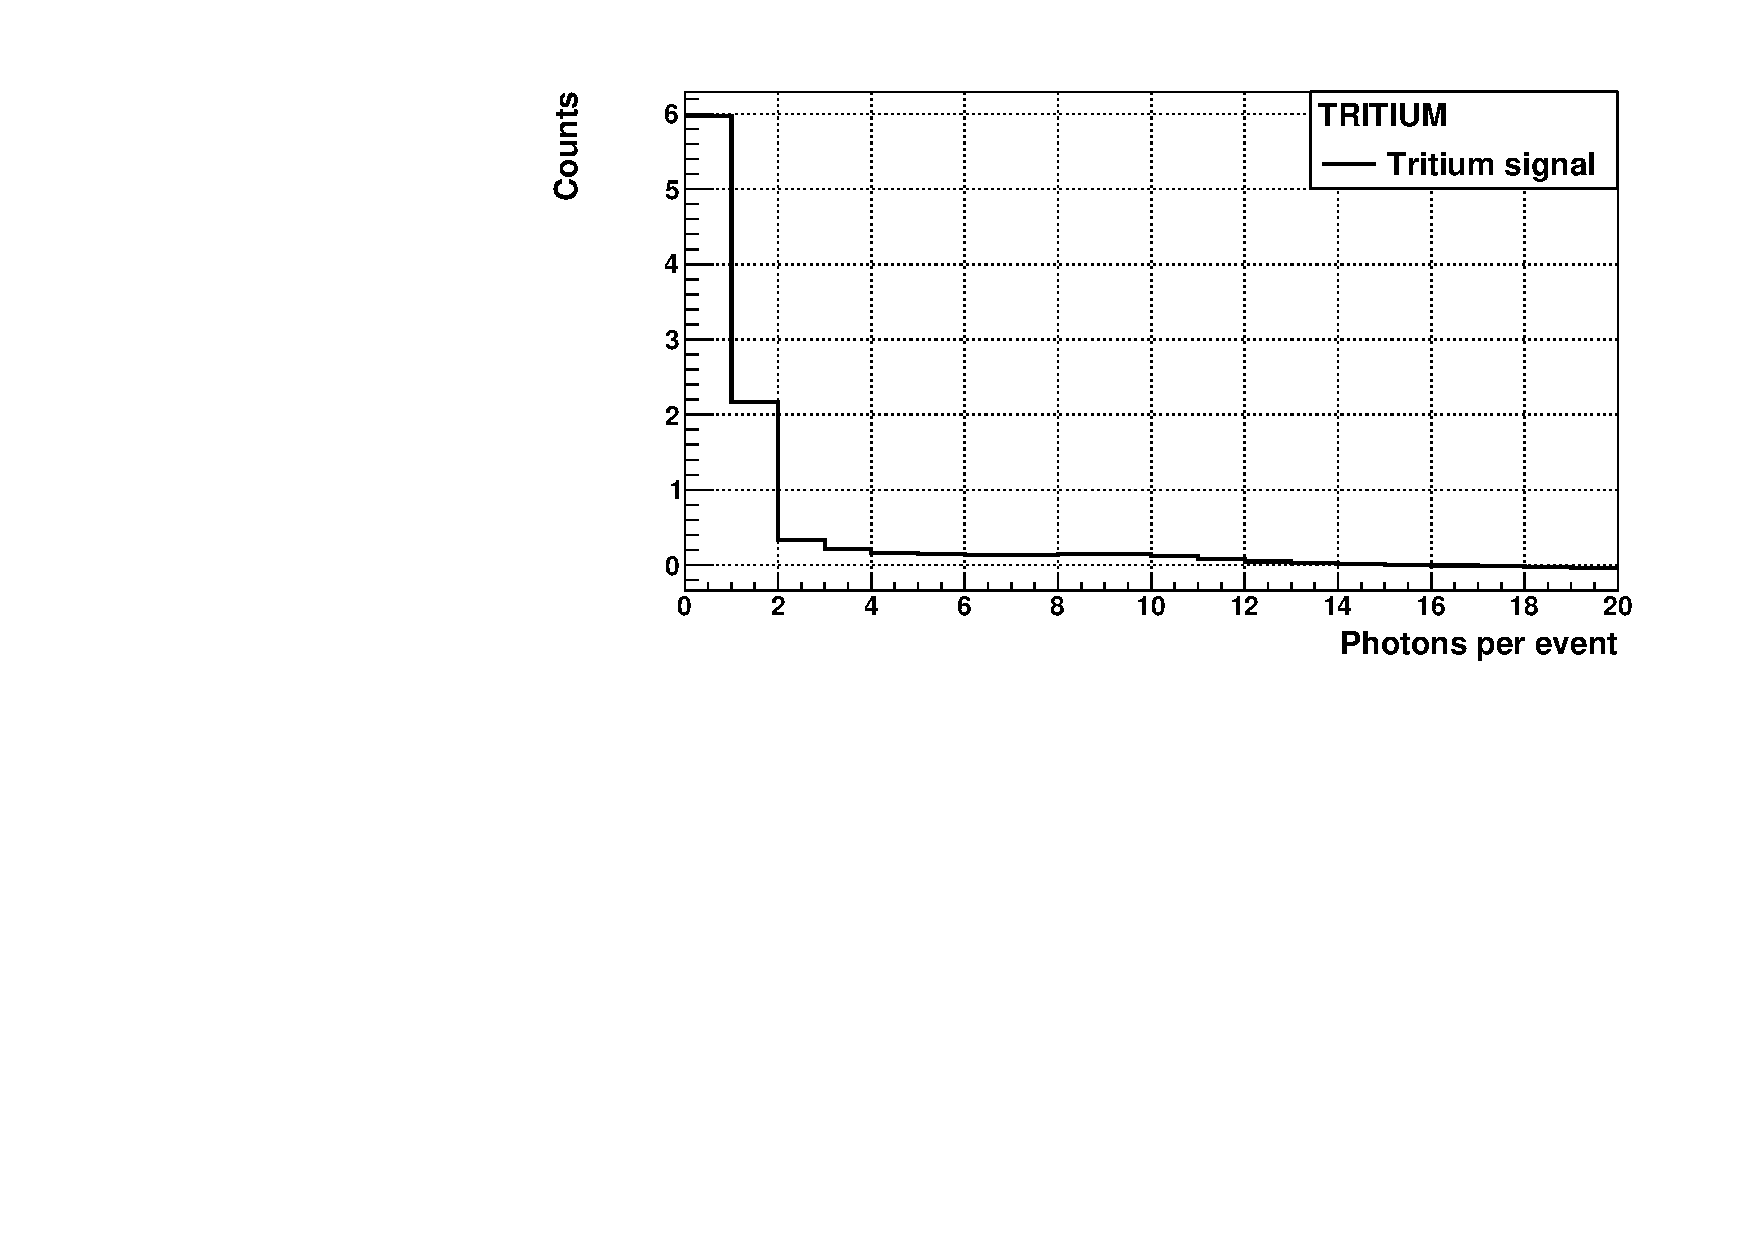
\includegraphics[width=\textwidth]{7ExperimentalResultsDetectors/71ExperimentalResultsLaboratory/714TRITIUMIFIC2/PhotonsPerTritiumEvent.pdf}  
    \caption{\label{subfig:TritiumSignalTRITIUMIFIC2}}
    \end{subfigure}
 \caption{a) Single photon distribution measured with TRITIUM-IFIC 2 prototype. b) Tritium energy spectrum measured with TRITIUM-IFIC 2 prototype in photons detected per event.}
 \label{fig:PhotonsPerTritiumEventIFIC2}
\end{figure}

%\begin{figure}[h]
%\centering
%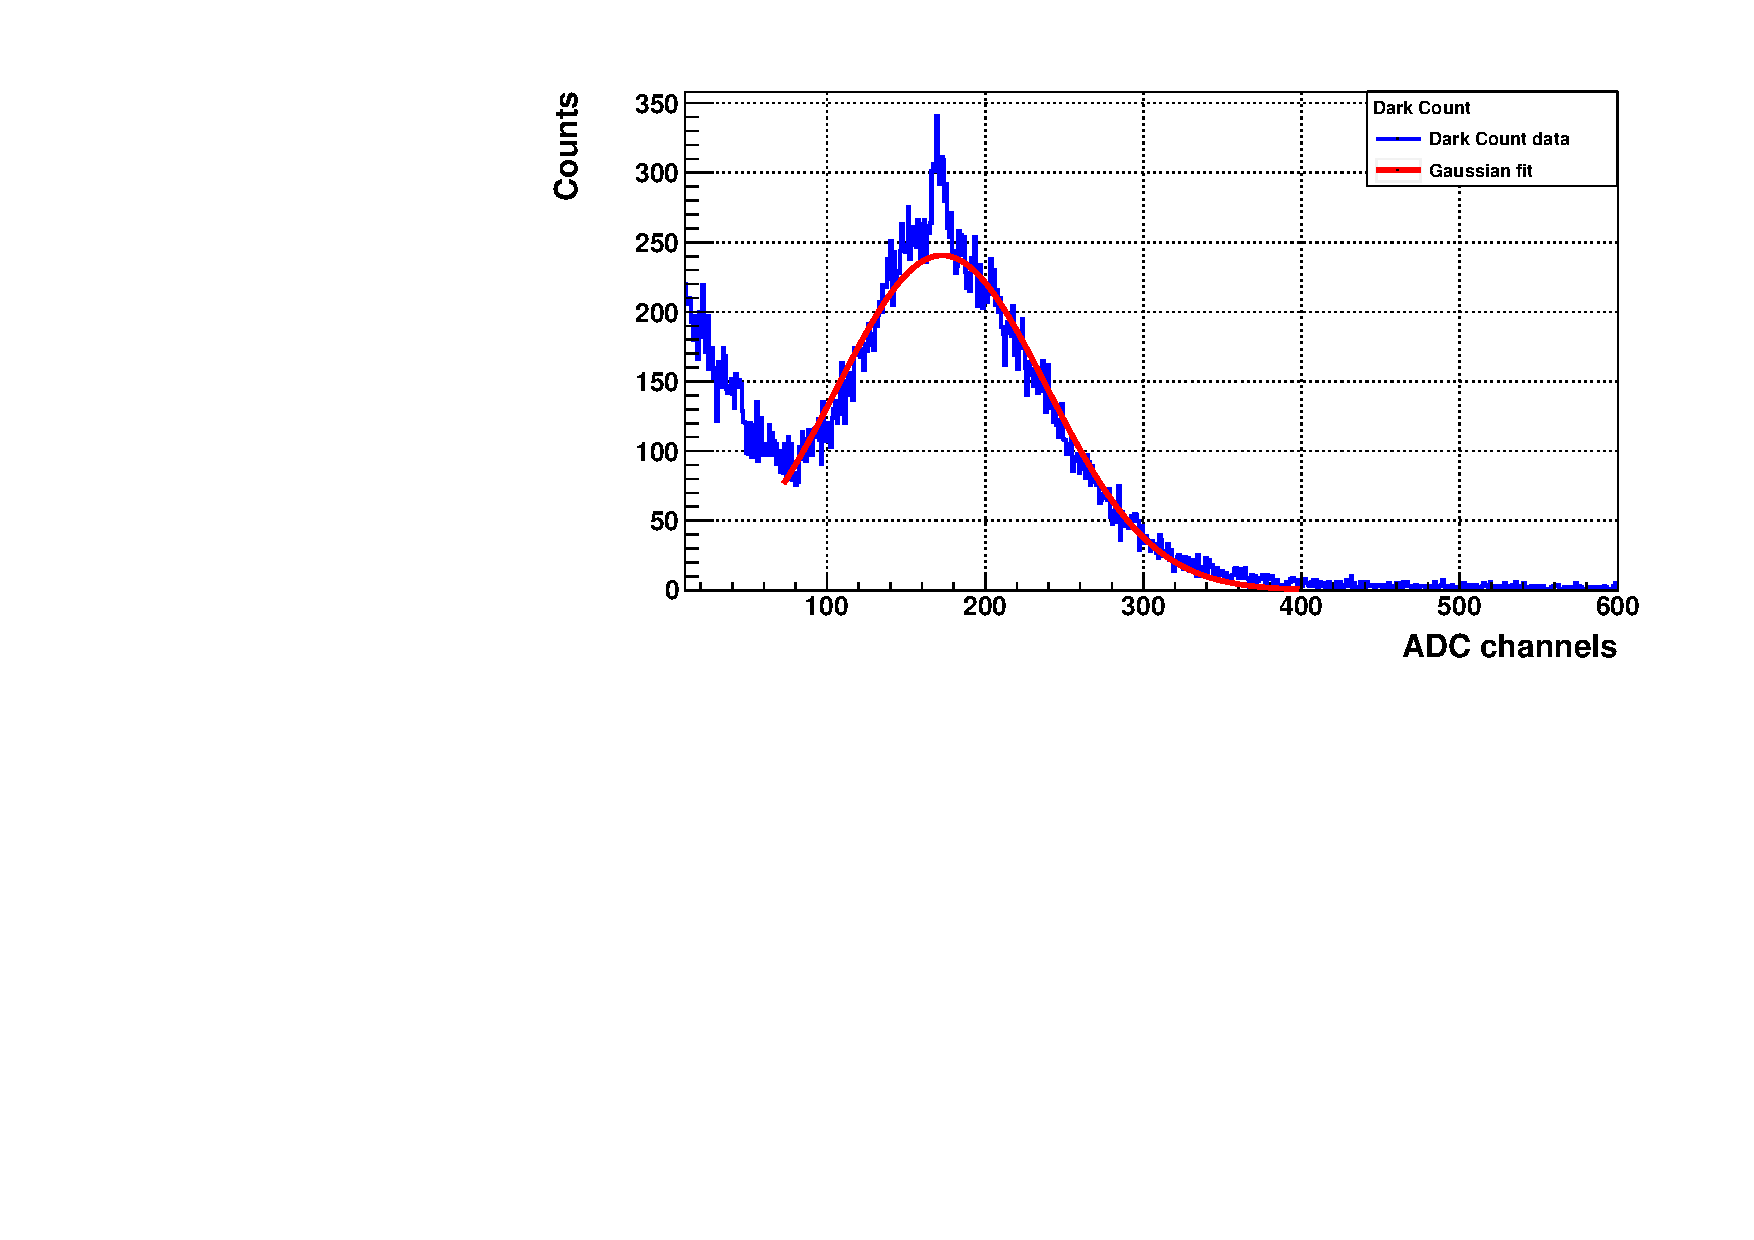
\includegraphics[scale=0.6]{7ExperimentalResultsDetectors/71ExperimentalResultsLaboratory/714TRITIUMIFIC2/SinglePhotonDistribution.pdf}
%\caption{Single photon energy distribution measured with the PMT used in TRITIUM-IFIC 2 prototype.\label{fig:SinglePhotonDistributionIFIC2}}
%\end{figure}

%\begin{figure}[h]
%\centering
%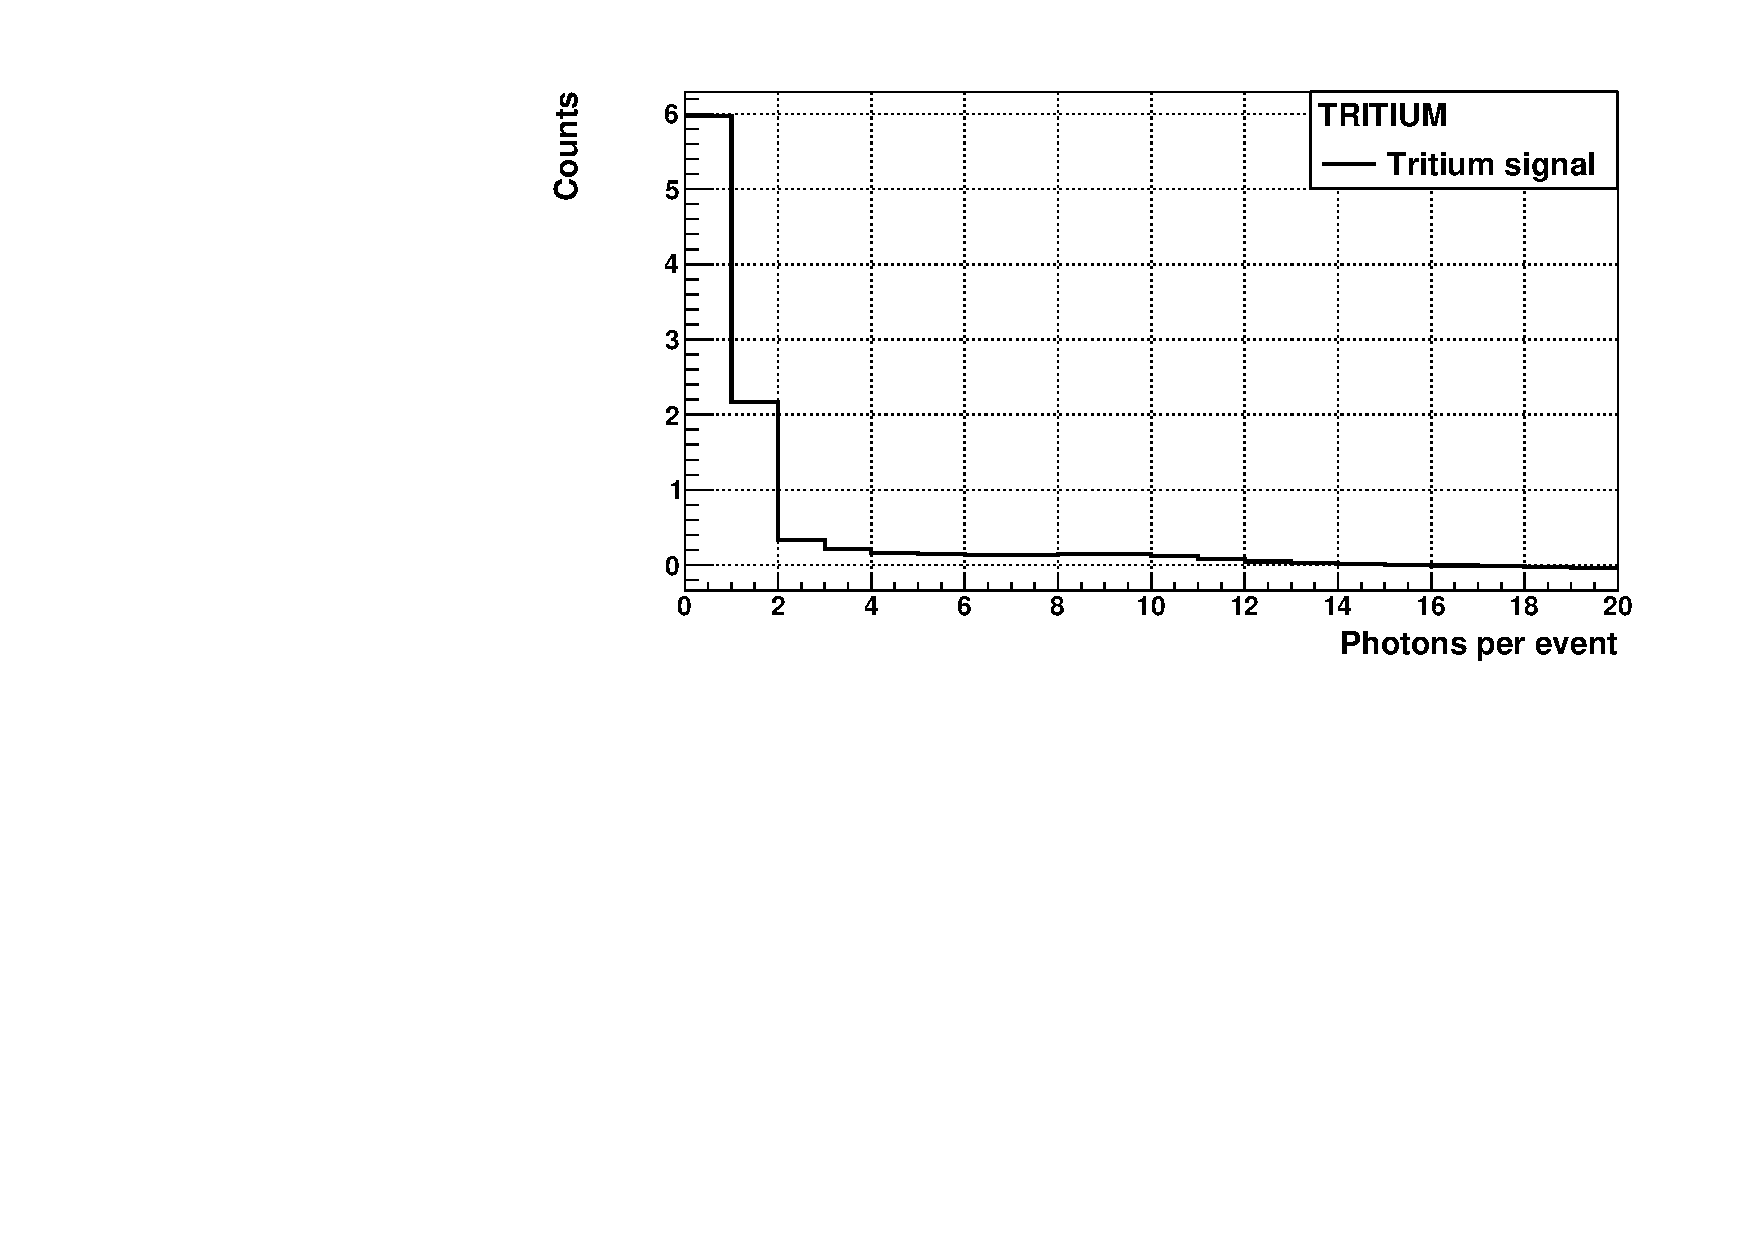
\includegraphics[scale=0.6]{7ExperimentalResultsDetectors/71ExperimentalResultsLaboratory/714TRITIUMIFIC2/PhotonsPerTritiumEvent.pdf}
%\caption{Tritium signal measured with the TRITIUM-IFIC 2 prototype and expressed in number of photones per tritium event detected.\label{fig:TritiumSignalTRITIUMIFIC2}}
%\end{figure}


%As can be seen, a maximum of $15$ photons are generated per tritium event, which corresponds to the best situation. To compare the value obtained with the expected one, the different energies and efficiencies involved are taken into account. Considering a maximum energy for the tritium electron detected, $18.6~\keV$, a scintillation yield of $8000~\text{ph}/\MeV$ for the fibers, a maximum collection efficiency for the fibers, $7\%/\meter$, the fiber length, $20~\cm$ (which increases the collection efficiency by a factor of 5), and the PMT efficiency, $29\%$, the maximum number of photons produced for a tritium event detected with TRITIUM-IFIC 2 prototype is $15$. As can be seen, this is perfectly in accordance with the measurement.

A monitoring of both prototypes, signal and background, were carried out during several months. The rates measured are shown in Figure \ref{fig:MonitorizationTRITIUMIFIC2}. No quenching of the signal was observed, indicating a stability the detector efficiency during 3 months for the signal and 6 months for the background. %Furthermore, it can be verified that the tritium activity used, $10~\kilo\becquerel/\liter$, is not the LDL of the TRITIUM-IFIC 2 prototype since both measurements, signal and background, are clearly separated along the time.

\begin{figure}[h]
\centering
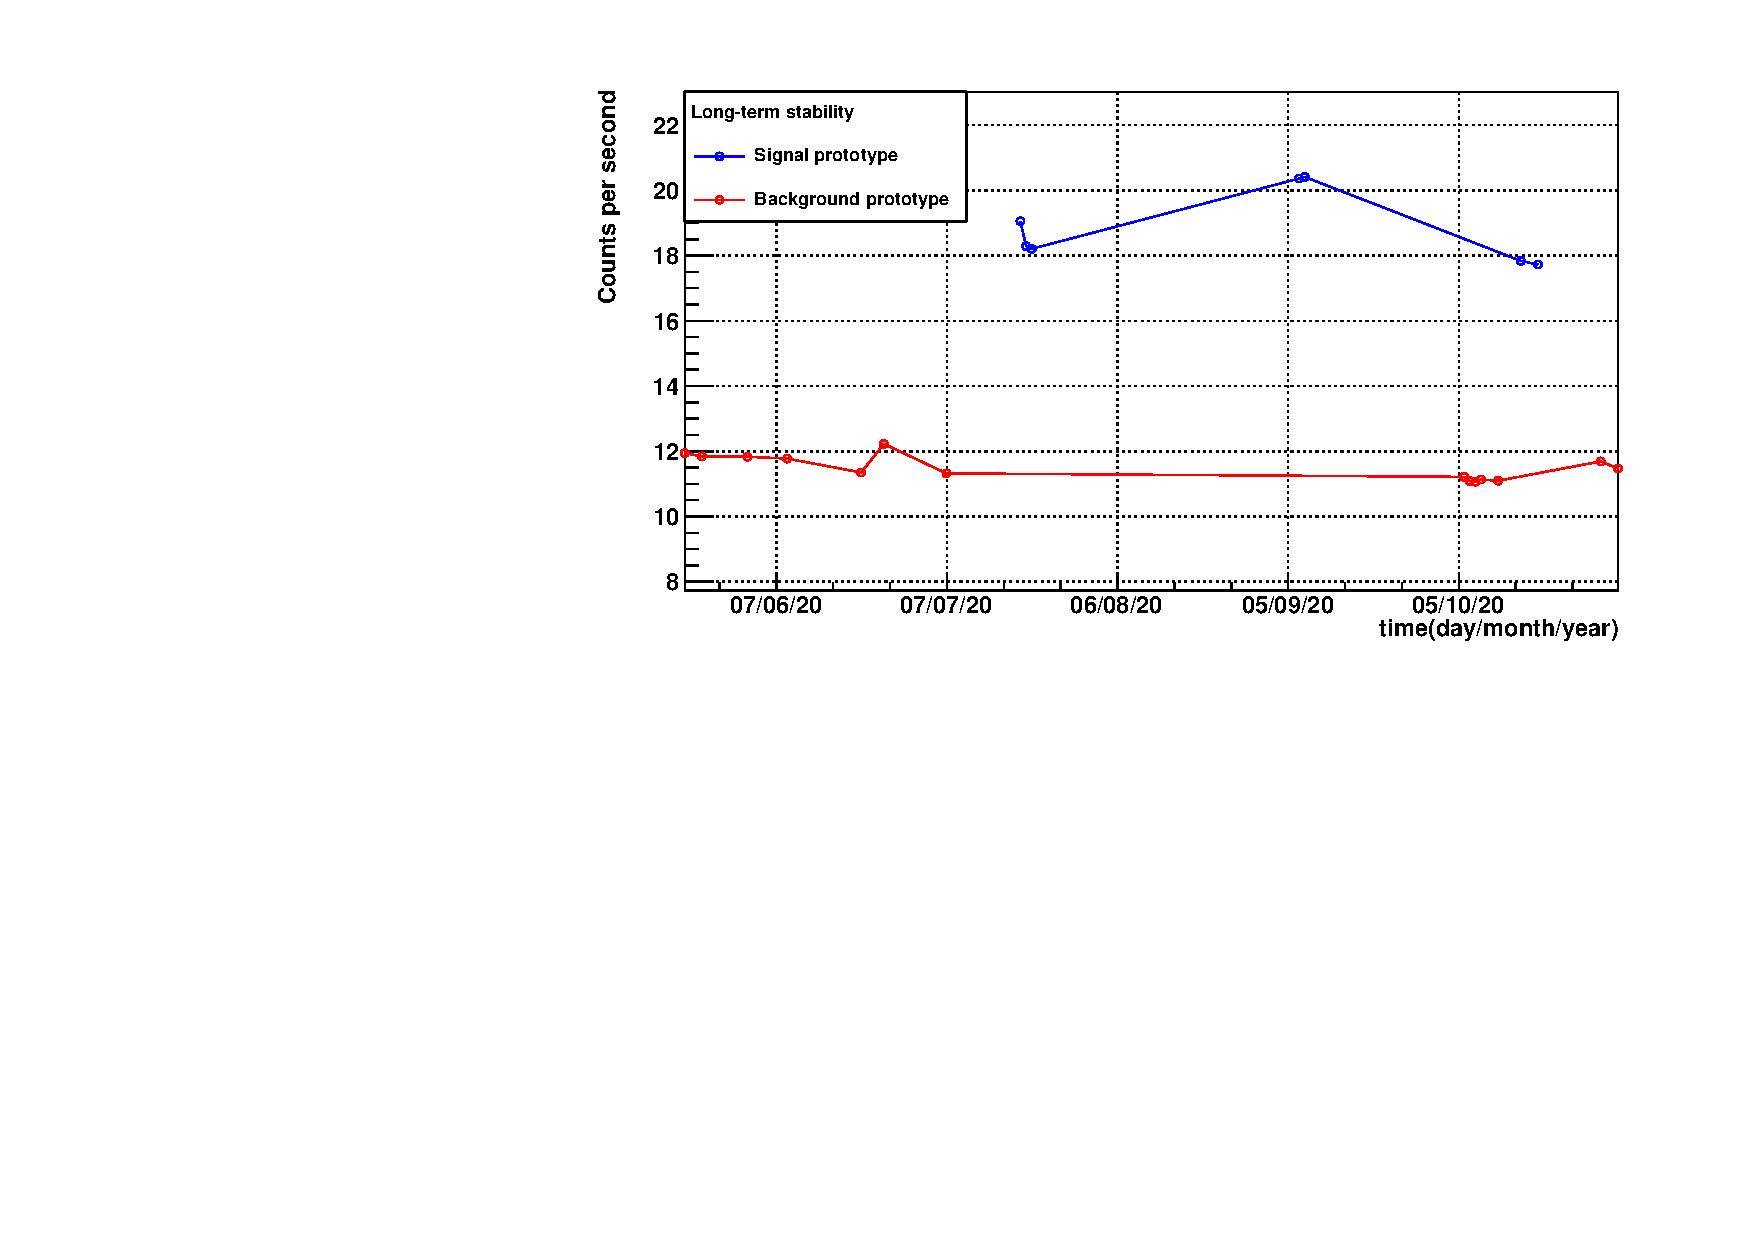
\includegraphics[scale=0.6]{7ExperimentalResultsDetectors/71ExperimentalResultsLaboratory/714TRITIUMIFIC2/Signal_Background_stability_ZOOM.pdf}
\caption{Signal and background rates for a long time measurement.\label{fig:MonitorizationTRITIUMIFIC2}}
\end{figure}


%ESTUDIAR EL LDL DEL DETECTOR CON LAS MEDIDAS TOMADAS!!!

%INCLUIR QUE NO SE HA CONSEGUIDO MEDIR 1kBq/L!!!


%Rellenar con uan actividad grande y volver a medir. 

%Vaciar el prototipo y rellenar con actividades más pequeñas. 1000 y 100 Bq/L.

%Comparar fondos en el laboratorio, caceres, almaraz, etc.

%Medir en el prototipo con SIPM.

%Menos fondo que con el prototipo de AVEIRO en laboratorio Aveiro pero más que en laboratorio extremadura!!!!!!!!!!!!!!!!!!!!